\thispagestyle{empty}
\section{Решения контрольной номер 1}

\subsection[2018-2019]{\hyperref[sec:kr_01_2018_2019]{2018-2019}}
\label{sec:sol_kr_01_2018_2019}

\begin{enumerate}
\item
Покажем, что все вероятности равны.
Пусть $ K $ — номер, под которым идёт Вася. Тогда вероятность того, что Вася
вытащит правильный билет равна вероятности того, что до него не вытащили правильный
билет, помноженная на вероятность того, что он вытащит верный (первое слагаемое)
плюс вероятность того, что до него уже вытащили один правильный билет, помноженная
на вероятность того, что он вытащит правильный билет.
По сути, это формула полной вероятности, где вероятность вытащить у Васи одинаковая
при разных условиях, так как он не знает, кто какой билет вытащил, а вероятности
условий (вытащили до него правильный билет или нет) разные.

Вероятность того, что Вася вытащит правильный билет равна
\[
\frac{\text{количество оставшихся хороших билетов}}{25-(K-1)},
\]

так как до Васи тянули ещё $К - 1$ студентов.

Начало второго слагаемого домножается на два, так как неизвестно, какой из двух
хороших билетов могли вытянуть до Васи. Следовательно, вероятность увеличивается
в два раза.

\begin{align*}
\P &= \frac{\binom{K-1}{23}}{\binom{K-1}{25}} \cdot \frac{2}{25-K+1} +  \frac{ 2 \cdot \binom{K-2}{23}}{\binom{K-1}{25}} \cdot \frac{1}{25-K+1} \\
&= \frac{23! \cdot (K-1)! \cdot (26-K)! \cdot2}{(K-1)! \cdot (24-K)! \cdot 25! \cdot (26-K)} + \frac{23! \cdot (K-1)! \cdot (26-K)! \cdot2}{(K-2)! \cdot (25-K)! \cdot 25! \cdot (26-K)} \\
&= \frac{2(25 - K)}{25 \cdot 24} + \frac{2(K-1)}{25 \cdot 24} \\
&= \frac{48}{25 \cdot 24} = \frac{2}{25}
\end{align*}

\item
\begin{enumerate}


\item
Зададим совместное распределение. Оно определяет все пересечения событий, то есть
когда события происходят одновременно. Тогда таблица имеет вид:

\begin{center}
	\begin{tabular}{ccc}
		\toprule
		$ \eta / \xi $ & $0$ & $1$ \\ \midrule
		$0$ & $\frac{4}{6} $ & $ \frac{1}{6} $ \\
		$1$ & $ \frac{1}{6} $  & 0 \\ \bottomrule
	\end{tabular}
\end{center}


\item
$\P(\xi = 1) \cdot \P(\eta = 1) = \frac{1}{16} \cdot \frac{1 }{16} = \frac{1}{36}$

$\P(\xi = 1 \cap \eta = 1) = 0 \Rightarrow \text{Величины не являются независимыми}$

\item

Зададим распределение $\xi + \eta$:

\begin{center}
\begin{tabular}{cccc}
\toprule
$\eta + \xi$ & $0$ & $1$ & $2$ \\
$\P(\eta + \xi = x)$ & $\frac{4}{6}$ & $\frac{2}{6}$ & $0$ \\ \bottomrule
\end{tabular}
\end{center}

\begin{figure}[ht!]
	\centering
	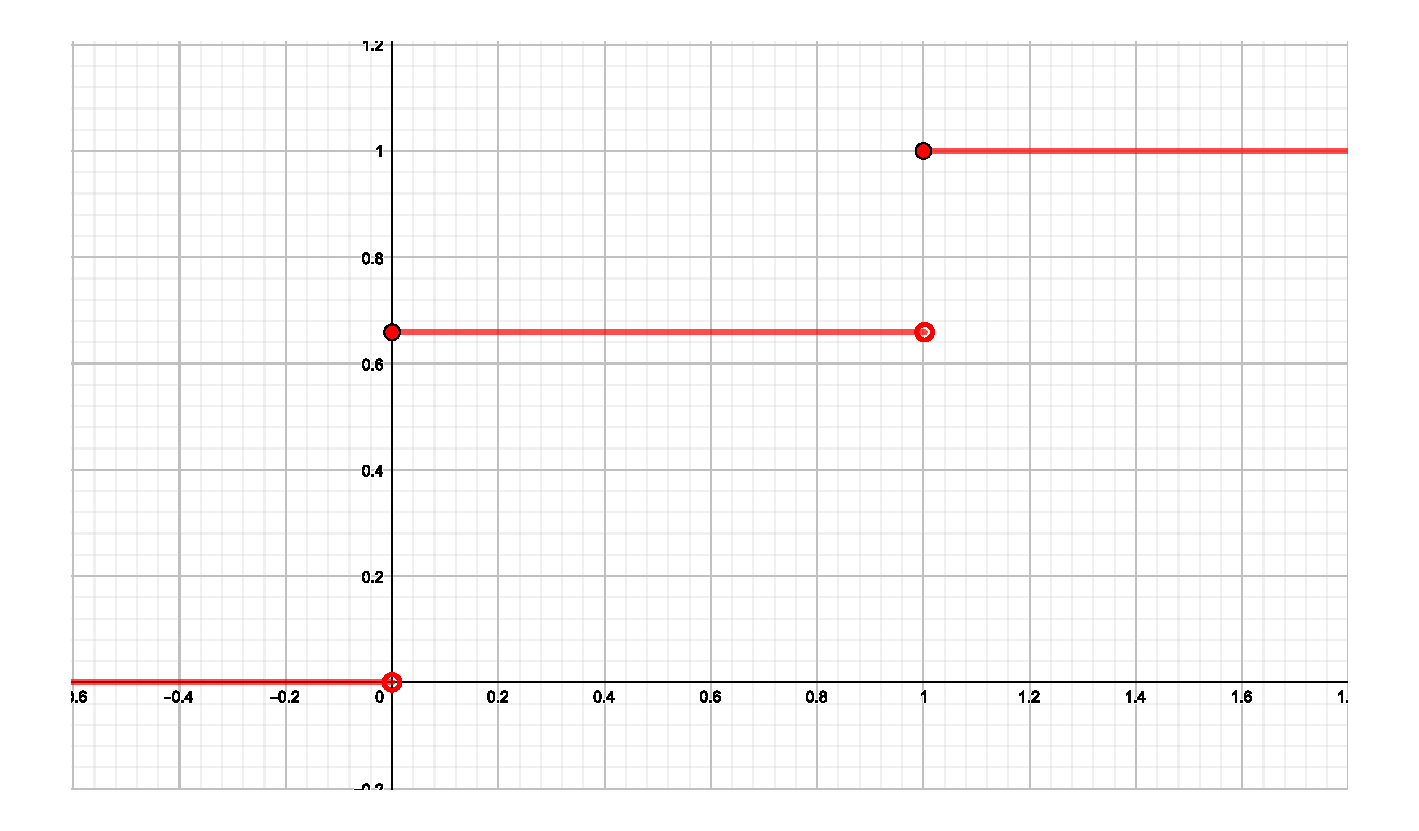
\includegraphics[width= 100mm]{images/kr1_2018.pdf}
	\caption{Функция распределения $\eta + \xi$}
	%\label{}
\end{figure}


\item
Зададим совместное распределение величин $\xi$ и $\xi + \eta$. Легко убедиться,
что случайные величины одновременно принимают соответствующие значения со следующими
вероятностями:

\begin{center}
	\begin{tabular}{ccc}
		\toprule
		$(\xi + \eta ) / \xi$ & $0$ & $1$ \\ \midrule
		$0$ & $\frac{4}{6} $ &$0$ \\
		$1$ & $\frac{1}{6}$  & $\frac{1}{6}$ \\
		$2$ & $0$  & $0$ \\
		\bottomrule
	\end{tabular}
\end{center}

Важно заметить, что когда, например, $\xi = 1$, то автоматически при
$\xi + \eta  = 1 \Rightarrow \eta = 0$ и вероятности легко находятся из частных распределений.
Из этой таблицы по формуле условной вероятности легко найти распределение:


\begin{center}
\begin{tabular}{ccc}
\toprule
$\xi | \xi + \eta = 1$ & $0$ & $1$ \\
$\P(\xi = x | \xi + \eta = 1)$ & $\frac{1}{2}$ & $\frac{1}{2}$ \\ \bottomrule
\end{tabular}
\end{center}
\end{enumerate}

\item
\begin{enumerate}
\item
\[
f_\xi(x) =
\begin{cases}
cx^2 , x \in [0;1] \\
0 , \text{иначе}
\end{cases}
\]

\[
\int_{0}^{1}cx^2 dx= \left. \frac{1}{3}c x^3 \right|_0^1 = \frac{1}{3} с = 1 \to c = 3
\]

\item
$\P(\xi = \frac{1}{2}) = 0$ по определению.

\[
\P\left(\xi \in \left[0, \frac{1}{3}\right]\right) = \left. \int_{0}^{\frac{1}{3}} 3x^2 dx = x^3 \right|_0^{\frac{1}{3}}  = \frac{1}{27}
\]
\item
\[
F_\xi(x) =
\begin{cases}
0 x < 0\\
x^3, x \in [0, 1]\\
1, x > 1
\end{cases}
\]

\item
$\P(\xi \in [\frac{1}{3}, \frac{3}{2}]) = \int_{\frac{1}{3}}^{1} 3x^2 dx = x^3 |_\frac{1}{3}^{1}  = 1 - \frac{1}{27} = \frac{26}{27}$

\item
$\P(\xi \le \frac{1}{2} |  \xi \ge \frac{1}{3}) = \frac{\P(\xi \le \frac{1}{2} ,  \xi \ge \frac{1}{3})}{\P(\xi \ge \frac{1}{3})}$

$\P(\xi \in [\frac{1}{3}, \frac{1}{2}])  = \int_{\frac{1}{3}}^{\frac{1}{2}} 3x^2 dx = x^3 |_\frac{1}{3}^{\frac{1}{2}} = \frac{1}{8} - \frac{1}{27} \approx 0.087$

\item
Так как функция плотности — парабола ветвями вверх $[0, 1]$, на котором она определена,
максимум будет достигаться на возрастающей части ветки, то есть в правом конце отрезка.
Следовательно, мода равна 1.

\item
$\E(\xi) = \int_{0}^{1} x 3x^2 dx = \frac{3}{4} x^4 |_0^1 = \frac{3}{4}$

\item

$\int_{0}^{q_{0.5}}3 x^2 dx = x^3  |_0^{q_{0.5}} = \frac{1}{2} \to q_{0.5} = \left(\frac{1}{2}\right)^\frac{1}{3}$
\end{enumerate}

\item
\begin{enumerate}
\item
$n = 12, q = \frac{1}{3}, p = \frac{2}{3}$


$12 \cdot \frac{2}{3}  - \frac{1}{2} \le \mu_0 \le 12 \cdot \frac{2}{3} + \frac{2}{3}$

$\frac{23}{3} \le \mu_0 \le \frac{26}{3}$

$ 7.6 \le \mu_0 \le 8.6 \to \mu_0 = 8$

\item

$\P(7  \text{ верных}) = \binom{12}{7} (1 - p)^{n - 7}\frac{12!}{7!5!}\left(\frac{1}{3}\right)^5\left(\frac{2}{3}\right)^7 \approx 0.19$

\item

Введём дополнительные переменные:
\begin{itemize}
\item $X$ — количество судей, которые вынесли обвинительный приговор
\item $A$ — принято верное решение
\item $B$ — подсудимый обвинён
\item $C$ — подсудимый виновен
\end{itemize}

\begin{align*}
\P(\text{Верный}) &= \P(\text{Обвинительный|Виновен})\P(\text{Виновен}) \\
&+  \P(\text{Не обвинительный | Невиновен})\P(\text{Невиновен})\\
&=\frac{\P(B\cap C)}{p} + \frac{\P(\bar{B}\cap \bar{C})}{1 - p} = \frac{2}{3}
\end{align*}

$\P(B|C) = P(X = 7|C) = \binom{12}{7}(1-p)^5p^7$

$\P(B|\bar{C}) = P(X = 7|C) = \binom{12}{7}(1-p)^7p^5$

$\P(X = 7) = \binom{12}{7}(1-p)^5p^2p + \binom{12}{7}(1-p)^7p^5(1-p) = \binom{12}{7}(1-p)^5p^5(p^3 + (1-p)^3)$

\item
$p = 0.17$

$\P(X = 7)  = \binom{12}{7}(1-0.17)^50.17^5(0.17^3 + (1-0.17)^3) \approx 0.025$

\end{enumerate}

\begin{enumerate}
\item
12 этажей, 11 человек.
Если указано, что они равновероятно выходят на любом этаже, то подъезд можно
представить, как отрезок, на который согласно равномерному распределению бросают
точку (человека), и он попадает в один из равновероятных 11 блоков. Тогда очевидно,
что вероятность того, что каждый попадёт в свой конкретный блок равна
\[
\left(\frac{1}{11}\right) ^{11} \approx 0
\]

\item
Исходя из той же логики, найдём условную вероятность того что все выйдут не выше
9-го, если известно, что они не вышли на первых пяти этажах. Будем подразумевать,
что первые пять этажей означает со 2 по 6. Тогда вероятность того, что все 11
человек выйдут на 7, 8 или 9, что является вероятностью пересечения события и
условия, будет равняться
\[
\left(\frac{3}{11}\right)^{11}
\]
Вероятность условия равна вероятности того что никто не выйдет на первых пяти
этажах равняется
\[
\left(\frac{5}{11}\right)^{11}
\]

Тогда условная вероятность равна
\[
\frac{\left(\frac{3}{11}\right)^{11}}{\left(\frac{5}{11}\right)^{11}} =  \left(\frac{3}{5}\right)^{11} \approx 0.003
\]
\end{enumerate}
\end{enumerate}




\subsection[2017-2018]{\hyperref[sec:kr_01_2017_2018]{2017-2018}}
\label{sec:sol_kr_01_2017_2018}

\begin{enumerate}
\item
\begin{enumerate}
\item События называются независимыми, если  $\P(A \cap B) = \P(A) \cdot \P(B)$
\item Запасёмся всеми нужными вероятностями:

$\P(A) = \frac{1}{2}$

$\P(B) = \frac{1}{3}$

$\P(C) = \frac{1}{2}$

$\P(A \cap C) = \frac{1}{3} $ — выпадет чётое число больше трёх

$\P(A \cap B)  = \frac{1}{6}$ — выпадет чётное число, кратное трём

$\P(A \cap C) = \frac{1}{6}$ — выпадет число, большее трёх и кратное трём

Теперь можно проверять независимость:

$\P(A \cap C) \neq \P(A) \cdot \P(C) \Rightarrow$  не являются независимыми

$ \P(A \cap B) = \P(A) \cdot \P(B) \Rightarrow$ являются независимыми

$ \P(B \cap C) = \P(B) \cdot \P(C) \Rightarrow$ являются независимыми

\end{enumerate}
\item
\begin{enumerate}
\item Количество возможных вариантов ТМ: $ C_{10}^2 $,  количество возможных
вариантов ЗМ: $ C_{24}^2 $. Количество их возможных сочетаний: $ C_{10}^2 \cdot C_{24}^2$,
где $ C_n^k = \frac{n!}{k!(n-k)!}$.
\item По классическому определению вероятностей, предполагая исходы равновероятными,
искомая вероятность равна $\frac{C_{16}^2}{C_{24}^2}$.
\item По тому же принципу:
\[
\frac{C_k^2}{C_{10}^2} = \frac{1}{15} \Rightarrow \frac{\frac{k!}{2!(k-2)!}}{\frac{10!}{2! \cdot 8!}} = \frac{1}{15} \Rightarrow \frac{(k-1)k}{2}\frac{ 2}{9 \cdot 10} = \frac{1}{15}
\]
Получаем квадратное уравнение вида $ k^2 - k - 6 = 0 $ с корнями $-2$ и $3$.
Так как $k$ не может быть отрицательным, ответ $3$.
\end{enumerate}
\item
\begin{enumerate}
\item Если эксперт отдаёт предпочтение Fit, то это можно интерпретировать как
«успех» в схеме Бернулли. Так как $\xi$ - количество успехов,
$ k \in [0;4]$, $p = \frac{1}{3} $, то
\[
\P(\xi = k) = C_n^k(p)^k(1-p)^{n-k}
\]

Большинство означает, что либо три, либо четыре эксперта выбрали Fit.
\[
\P(\xi = 3) = C_4^3\left(\frac{1}{3}\right)^3 \left(\frac{2}{3}\right)^{1} = \frac{8}{81}
\]
\[
\P(\xi = 4) = C_4^4\left(\frac{1}{3}\right)^4 \left(\frac{2}{3}\right)^{0} = \frac{1}{81}
\]
\[
\P( \xi > 2) =  \frac{9}{81}
\]
\item Аналогично:

\[ \P(\xi = 0) = C_4^0\left(\frac{1}{3}\right)^0 \left(\frac{2}{3}\right)^{4} = \frac{16}{81}\]

\[ \P(\xi = 1) = C_4^1\left(\frac{1}{3}\right)^1 \left(\frac{2}{3}\right)^{3} = \frac{32}{81}\]

\[ \P(\xi = 2) = C_4^2\left(\frac{1}{3}\right)^2 \left(\frac{2}{3}\right)^{2} = \frac{24}{81}\]

\begin{figure}[h!]
    \noindent\centering{
    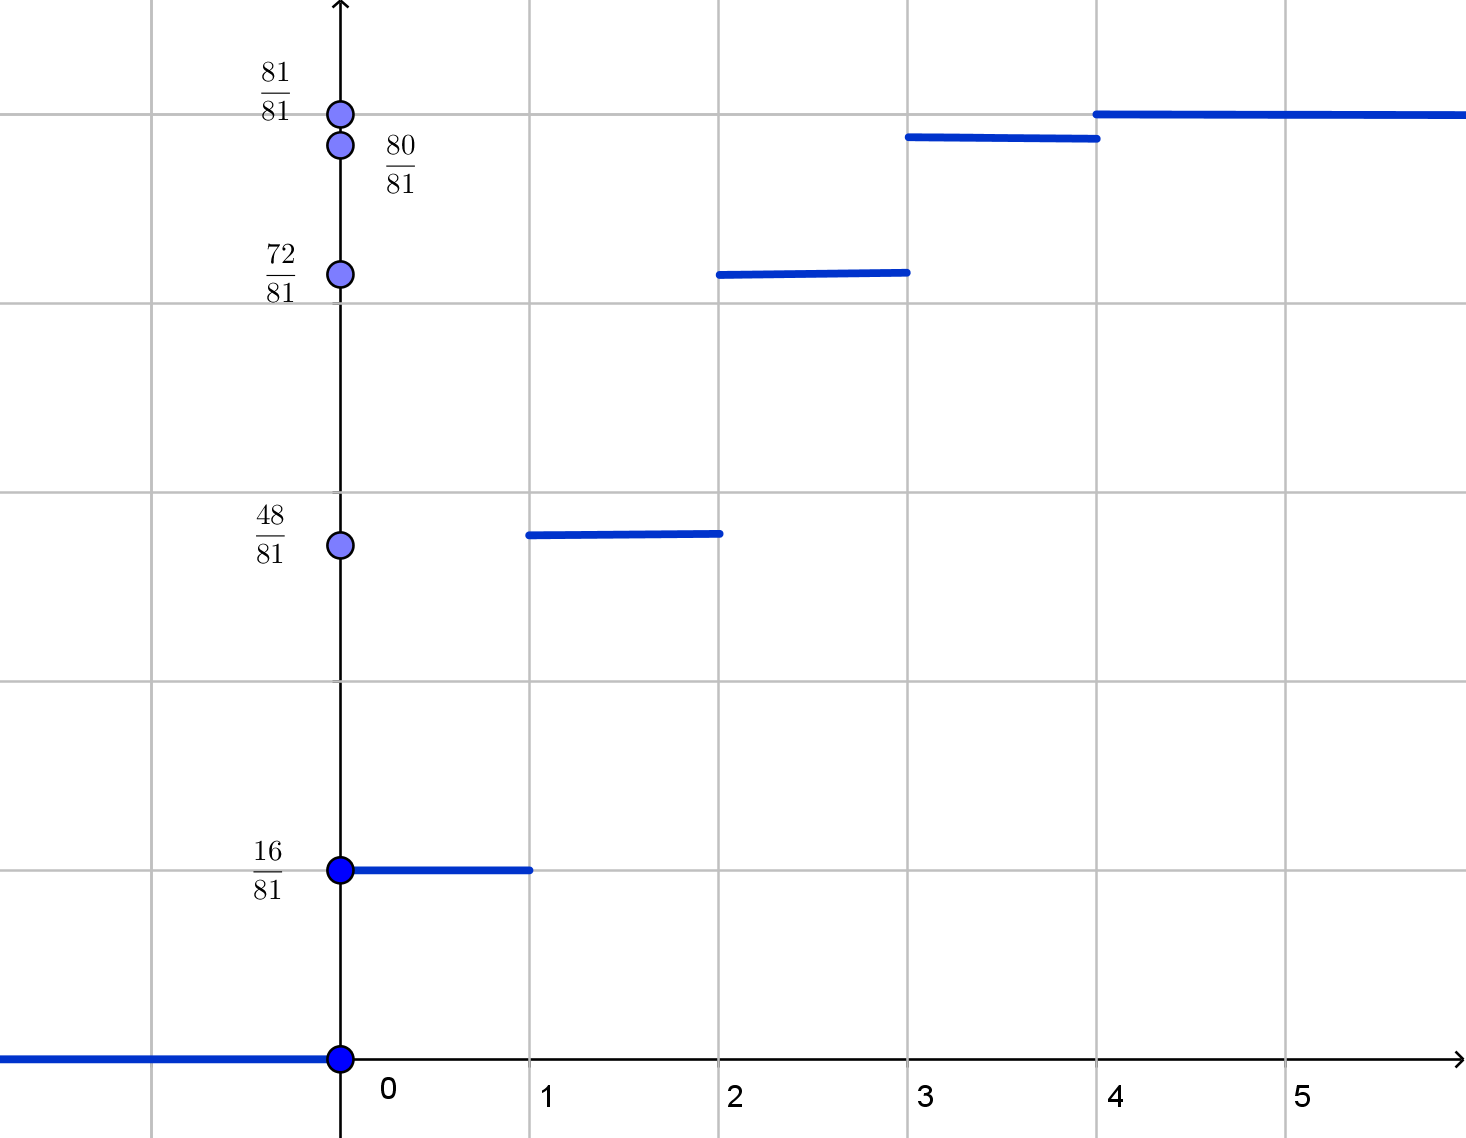
\includegraphics[width=80mm]{images/kr1_2017_3.png}
    }
    \caption{Функция распределения}
    \label{cdf_kr2017}
\end{figure}

\item Все вероятности посчитаны, видим, что наибольшая достигается при $\xi=1$.
\item $\E(X) = np = \frac{4}{3} $, $ \Var(X) = npq = \frac{8}{9}$
\end{enumerate}
\item
\begin{enumerate}
\item Так как указано, что цена сметаны распределена равномерно на отерзке
$[250, 1000]$, максимальное значение цены — $1000$, это и есть необходимая сумма.
\item Вспомним, что функция распределения $F(x) = \P(X \leq x)$, нужно найти
такой $x$, что $ \P(X \leq x)=0.9$:
\[
0.9 = 1 - \exp({-x^{2}}) \Rightarrow \exp(-x^{2}) = 0.1 \Rightarrow -x^2 = \ln(0.1)  \Rightarrow x=  \sqrt{-\ln(0.1)}
\]
\item Взяв производную от функции распределения списка без сметаны, получим функцию
плотности:
\[
f_X(x) =
\begin{cases}
2x\exp(-x^2) & x \ge 0 \\
0 & \text{иначе}
\end{cases}
\]
Найдём математическое ожидание:
\[
\int_{0}^{+\infty}2x^2\exp({-x^2}) dx = -x \exp({-x^2})\big|_0^{+\infty}
+ \int_{0}^{+\infty}\exp({-x^2}) dx = \frac{\sqrt{\pi}}{2}
\]
\item Математическое ожидание суммы случайных величин равно сумме математических
ожиданий случайных влечин, если они существуют. Математическое ожидание от цены
сметаны равно: $ \frac{1000 + 250}{2} = 625$.
Математическое ожидание списка без сметаны было найдено в предыдущем пункте, его
осталось перевести в рубли. Получаем ответ: $ 625 + \frac{\sqrt{\pi}}{2} \cdot 1000 $.
\item Так как обе величины имеют абсолютно непрерывные распределения, вероятность
попасть в конкретную точку равна нулю.
\end{enumerate}
\item
\begin{enumerate}
\item $\P(\text{детектор показал ложь и подозреваемый лжёт}) = 0.9 \cdot 0.1 + 0.1 \cdot 0.95 = 0.185$
\item $\P(\text{невиновен}|\text{детектор показал ложь}) = \frac{0.9\cdot0.1}{0.185} = \frac{90}{185}$
\item $\P(\text{эксперт точно выявит преступника}) = (0.9)^9 \cdot 0.95$
\item $\P(\text{эксперт ошибочно выявит преступника}) = 9 \cdot 0.1 \cdot 0.9^8\cdot 0.05$
\end{enumerate}
\end{enumerate}


\subsection[2016-2017]{\hyperref[sec:kr_01_2016_2017]{2016-2017}}
\label{sec:sol_kr_01_2016_2017}

\begin{enumerate}
\item
\begin{enumerate}
\item Возможны четыре равновероятные ситуации:
\[
\P(\text{ММ}) = \P(\text{МД}) = \P(\text{ДМ}) = \P(\text{ДД}) = 1/4
\]

Посчитаем условную вероятность:
\[
\P(B \mid A) = \frac{\P(B \cap A)}{\P(A)} = \frac{\P(\text{МД, ДМ})}{\P(\text{ДМ, МД, ДД})} = \frac{2/4}{3/4} = \frac{2}{3}
\]

\item События $A$ и $B$ называются независимыми, если $\P(A \cap B) = \P(A) \cdot \P(B)$

В нашем случае: $\P(A \cap B) = \P (\text{МД, ДМ}) = 2/4$,
$\P(A) \cdot \P (B) = 3/4 \cdot 3/4$.

Следовательно, $\P(A \cap B) \neq \P(A) \cdot \P (B)$,
значит, события $A$ и $B$ не являются независимыми.
\end{enumerate}

\item Пусть событие $A_i$ означает, что $i$-ый узел системы дал сбой,
а событие $B_N$, что вся система дала сбой.

В условии сказано, что $\P(A_i) = 10^{-6}$,
а найти нужно такое максимальное $N \in \mathbb{N}$, при котором

\[
\P(B_N) \leq \frac{1}{10^2}
\]

\begin{align*}
\P(B_N) &= \P\left(\cup_{i=1}^n A_i\right) = 1 - \P (\left(\cup_{i=1}^n A_i\right)^c) \\
&\stackrel{\text{ф-ла де Моргана}}{=} 1 - \P \left(\cap_{i=1}^N A_i^c\right) \stackrel{A_1, \ldots, A_N \text{– независ.}}{=} 1 - \P(A_1^c) \cdot \ldots \cdot \P(A_N^c) \\
&= 1 - \left(1-\frac{1}{10^6}\right)^N
\end{align*}
Чтобы найти такое максимальное $N \in \mathbb{N}$, надо решить следующее неравенство
\begin{align*}
& 1 - \left(1-10^{-6}\right)^N \leq 10^{-2} \\
& 1 - 10^{-2} \leq \left(1-10^{-6}\right)^N \\
& \ln\left(1 - 10^{-2}\right) \leq N \ln \left(1 - 10^{-6}\right) \\
& N \leq \frac{\ln\left(1 - 10^{-2}\right)}{ \ln \left(1 - 10^{-6}\right)} \approx 10050.33
\end{align*}
Значит, максимальное $N$ равно $10050$.

\item Введём обозначения для событий.
Пусть $A$ означает, что человек имеет заболевание лёгких,
а $B$, что человек работал в шахте.

В условии сказано, что $\P(B \mid A) = 0.22$, $\P(B \mid A^c) = 0.14$, $\P(A) = 0.04$.
\begin{enumerate}
\item Нужно найти
\[
\P(A \mid B) = \frac{\P(A\cap B)}{\P (B)} = \frac{\P(B|A)\P(A)}{\P(B)}
\]
Для этого с помощью формулы полной вероятности посчитаем
\[
\P (B) = \P (B \mid A) \P(A) + \P (B \mid A^c) \P (A^c) = 0.22 \cdot 0.04 + 0.14 \cdot 0.96 = 0.1432
\]
Осталось подставить значения:
\[
\P(A \mid B) = \frac{0.22 \cdot 0.04}{0.1432} \approx 0.0615
\]

\item Все необходимые значения для второго пункта у нас есть,
осталось применить формулу условной вероятности:
\begin{align*}
\P  (A \mid B^c) &=  \frac{\P(A\cap B^c)}{\P (B^c)} =  \frac{\P (B^c \cap A)}{\P(A)} \cdot \frac{\P(A)}{\P (B^c)} = \P (B^c \mid A) \cdot \frac{\P(A)}{\P (B^c)} \\
&= (1-\P (B \mid A)) \cdot \frac{\P(A)}{1-\P (B)} = (1-0.22) \cdot \frac{0.04}{1-0.1432} \approx 0.0364
\end{align*}
\end{enumerate}
\item Введём индикатор события «Петя дал верный ответ на $i$-ый вопрос»:
\[
X_i =
\begin{cases}
1, & \text{если на } i \text{-ый вопрос теста Петя дал верный ответ} \\
0, & \text{иначе}
\end{cases}
\]

Заметим, что $X_i \sim Be\left(p = 1/5 \right)$, $X_1, \ldots, X_{17}$ – независимы,
$X = X_1 + \ldots + X_{17}$ – общее число верных ответов,
$X \sim Bin\left(n=17, p=1/5\right)$.

\begin{enumerate}
\item Наибольшее вероятное число правильных ответов $m_0$ может быть нвйдено по формуле:
\begin{enumerate}
\item[1)] если число $(n\cdot p - q)$ – не целое, где $q:=1-p$, то
\[
m_0 = [np-q] +1,
\]
\item[2)] если число  $(n\cdot p - q)$ – целое, то наиболее вероятных значений $m_0$ два:
\[
m_0' = np-q \text{ и } m_0'' = np-q+1
\]
\end{enumerate}
Итак, поскольку $np-q = 17\cdot\frac{1}{5} - \frac{4}{5} = 2.6$ – не целое, наиболее вероятное число верных ответов $m_0$ может быть найдено по формуле из пункта (1):
\[
m_0 = [np-q] +1 = [2.6] + 1 = 3
\]
\item \[\E(X) = np = 17 \cdot \frac{1}{5}=3.4\]

\[\Var(X) = npq = 17 \cdot \frac{1}{5} \cdot \frac{4}{5} = 2.72\]

\item
\begin{align*}
\P (\text{у Пети «отлично»}) &= \P (X\geq 15) = \P (X = 15) + \P (X= 16) + \P (X = 17) \\
& = C^{15}_{17} \cdot \left(\frac{1}{5}\right)^{15} \cdot \left(\frac{4}{5}\right)^2 + C^{16}_{17} \cdot \left(\frac{1}{5}\right)^{16} \cdot \left(\frac{4}{5}\right)^1 + C^{17}_{17} \cdot \left(\frac{1}{5}\right)^{17} \cdot \left(\frac{4}{5}\right)^0 \\
&= 136 \cdot \frac{16}{5^{17}} + 17 \cdot \frac{4}{5^{17}} + \frac{1}{5^{17}} \approx 2.94 \cdot 10^{-9}
\end{align*}
\item Рассмотрим первый вопрос теста. Петя может выбрать первый ответ с вероятностью $1/5$, и Вася
может выбрать первый ответ с вероятностью $1/5$. Тогда они оба выберут одинаковый ответ с вероятностью $1/25$.
Вариантов ответа в каждом вопросе $5$, значит, вероятность совпадения ответа в одном вопросе равна $1/5$.
Всего вопросов 17, тогда получаем
\[
\P(\text{все ответы Пети и Васи совпадают}) = \left(\frac{1}{5}\right)^{17}
\]

\end{enumerate}
\item Введём случайную велчину $\eta$, которая означает число потенциальных покупателей,
с которыми контактировал продавец оборудования. По условию задачи, $\eta$ имеет
таблицу распеределения:
\begin{center}
\begin{tabular}{ccc}
\toprule
$y$ & $ 1 $ & $2$ \\
$\P(\eta = y)$ & $1/3$ & $2/3$ \\ \bottomrule
\end{tabular}
\end{center}
Случайная величина $\xi$ может принимать значения $0, 50000$ и $100000$
\begin{enumerate}

\item Найдём $\P (\xi = 0 )$. По формуле полной вероятности, имеем:
\begin{align*}
\P (\xi = 0) &= \P (\xi = 0 \mid \eta = 1 ) \cdot \P ( \eta = 1 ) + \P (\xi = 0 \mid \eta = 2 )  \cdot \P ( \eta = 2 ) \\
&= 0.9 \cdot \frac{1}{3} + 0.9\cdot0.9 \cdot \frac{2}{3} = 0.84
\end{align*}

\item Найдём $\P (\xi = 50000 )$ и $\P (\xi = 100000 )$ :
\begin{align*}
\P (\xi = 50000 ) &= \P (\xi = 50000 \mid \eta = 1 ) \cdot \P ( \eta = 1  ) +  \P (\xi = 50000 \mid \eta = 2 ) \cdot  \P ( \eta = 2 ) \\
&= 0.1 \cdot \frac{1}{3} + 2 \cdot 0.1 \cdot 0.9 \cdot \frac{2}{3} = 0.15(3)
\end{align*}
\begin{align*}
\P (\xi = 100000 ) &=  \P (\xi = 100000 \mid \eta = 1 ) \cdot \P ( \eta = 1 ) +  \P (\xi = 100000 \mid \eta = 2 ) \cdot  \P ( \eta = 2  ) \\
&= 0 \cdot \frac{1}{3} + 0.1\cdot 0.1  \cdot \frac{2}{3} = 0.00(6)
\end{align*}
Таблица распределения случайной величина $\xi$ имеет вид:

\begin{center}
\begin{tabular}{cccc}
\toprule
$x$ & $ 0 $ & $50\,000$ & $100\,000$ \\
$\P(\xi = x)$ & $0.84$ & $0.15(3)$ & $0.00(6)$ \\ \bottomrule
\end{tabular}
\end{center}

Тогда функция распределения случайной величины $\xi$ имеет вид:
\[
F_{\xi} (x) =
\begin{cases}
0 & \text{при } x<0 \\
0.84 & \text{при } 0 \leq x < 50\,000 \\
0.84 + 0.15(3) & \text{при } 50\,000
\leq x < 100\,000 \\
1 & \text{при } x > 100\,000
\end{cases}
\]
Опр.: $F_{\xi} = \P (\xi \leq x ), x \in \mathbb{R}$
\item \[
\E (X) = 0 \cdot 0.84 + 50\,000 \cdot 0.15(3) + 100\,000 \cdot 0.00(6) = 8\,333.(3)
\]
\begin{align*}
\Var(X) &= (0 - 8\,333.(3))^2 \cdot 0.84 + (50\,000-8\,333.(3))^2 \cdot 0.15(3) \\
&+ (100\,000 - 8\,333.(3))^2 \cdot 0.00(6) = 380\,555\,555.(5)
\end{align*}
\end{enumerate}
\item
\begin{enumerate}
\item $ f_{\xi} (x)=
\begin{cases}
\frac{1}{b} & \text{при } x \in [0, b] \\
0 & \text{при } x \notin [0, b]
\end{cases}
$
\item  Известно, что если $\xi \sim U[a, b]$, то $\E (\xi) = \frac{a+b}{2}$. Стало быть, из уравнения $\E (\xi) = 1$ получаем $\frac{b}{2} = 1$,  то есть $b=2$.
\item Известно, что если $\xi \sim U[a, b]$, то $\Var (\xi) = \frac{(b-a)^2}{12}$. Значит, $\Var (\xi) = \frac{2^2}{12} = \frac{1}{3}$
\item Воспользуемся формулой $\P (\xi \in B ) = \int_B f_{\xi} (x) dx$. Имеем:
\[
\P (\xi > 1 ) = \P (\xi \in (1, + \infty) ) = \int_{1}^{+ \infty} f_{\xi} (x) dx = \int_{1}^{2} \frac{1}{2} dx = \frac{1}{2}
\]
\item Требуется найти такое минимальное число $q_{0.25}$, что $\int_{-\infty}^{q_{0.25}} f_{\xi} (x) dx = 0.25$. Итак:
\[
\int_{-\infty}^{q_{0.25}} f_{\xi} (x) dx = 0.25 \Leftrightarrow \int_{-\infty}^{q_{0.25}} \frac{1}{2} dx = 0.25 \Leftrightarrow \frac{1/2}{q_{0.25}} = 0.25 \Leftrightarrow
\]
\[
q_{0.25} = 2 \cdot 0.25 = 0.5
\]
\item
\begin{align*}
\E \left((\xi - \E(\xi))^{2017} \right) &= \int_{-\infty}^{+\infty} (x- \E(\xi) )^{2017} \cdot f_{\xi} (x) dx = \int_{-\infty}^{+\infty} (x-1)^{2017} f_{\xi} (x) dx \\
&= \int_{0}^{2} (x-1)^{2017} \cdot \frac{1}{2} dx = \frac{(x-1)^{2018}}{2018} \cdot \frac{1}{2} \bigg\rvert_{x=0}^{x=2} =0
\end{align*}
\item $F_{\xi} (x) =
\begin{cases}
0 & \text{при } x < 0 \\
\frac{x}{2} & \text{при } 0 \leq x \leq 2 \\
1 & \text{при } x > 2
\end{cases}
$
\item Согласно условиям задачи, время до прихода 1-го поезда есть $\xi$; время до прихода 2-го поезда равно $\xi + b$; время до прихода 3-го (заветного) поезда есть $\xi + 2b$. Таким образом, Марья Ивановна в среднем ожидает «своего» поезда $\E (\xi + 2b) = 1 + 2b = 1 + 2 \cdot 2 = 5 $ минут. При этом $\Var (\xi + 2b) = \Var (\xi) = 1/3$
\item[к)] Пусть $\tau$ – наименьший номер поезда без «подозрительных лиц». По условию задачи, таблица распределения случайной величины $\tau$ имеет вид:

\begin{center}
\begin{tabular}{cccccc}
\toprule
$t$ & $ 1 $ & $2$ & $3$ & $4$ & \ldots \\
$\P(\tau = t)$ & $1/4$ & $3/4\cdot1/4$ & $(3/4)^2 \cdot 1/4$ & $(3/4)^3 \cdot 1/4$ & \ldots\\ \bottomrule
\end{tabular}
\end{center}

То есть случайная величина $\tau$ имеет геометрическое распределение с параметром $p=1/4$ $(\tau \sim G(p=1/4))$.

Несложно сообразить, что время ожидания Глафирой Петровной «своего» поезда составляет: $\eta := \xi + b(\tau- 1)$. Стало быть, $\E (\eta) = \E (\xi) + b \cdot (\E(\tau)-1)  = 1 + 2 \cdot (4-1) = 7$ минут.

Здесь мы воспользовались тем фактом, что если $\eta \sim G(p)$, то $\E (\eta) = 1/p$
\item[и)] Найдём теперь вероятность $\P (\eta \geq 5 )$. Для нахождения искомой вероятности воспользуемся формулой полной вероятности:
\[
\P (\eta \geq 5) = \P(\eta \geq 5, \tau < 3) + \P(\eta \geq 5, \tau = 3) +
\P(\eta \geq 5, \tau > 3)
\]

Если Глафира уехала на первом или втором поезде,
то ждать больше 5 минут она не могла, то есть $\P(\eta \geq 5, \tau <3)=0$.

Если Глафира уехала на третьем поезде, то чтобы ждать больше пяти минут,
ей нужно ждать первый поезд больше минуты,
то есть $\P(\eta \geq 5, \tau = 3)=0.5 \P(\tau = 3)$.

Если Глафира уехала на четвертом поезде или позже, то она точно ждала больше 5 минут,
$\P(\eta \geq 5, \tau >3)=\P(\tau>3)$.

\[
\P(\eta \geq 5) = 0.5\P(\tau = 3) + \P(\tau > 3) = 0.5 \cdot (3/4)^2 \cdot (1/4) + (3/4)^3 = 63 / 128
\]

\end{enumerate}
\item Пусть $\xi$ — случайная величина, обозначающая число остановок лифта. Предствим её в виде суммы $\xi = \xi_2 + \ldots + \xi_{10}$, где $\xi_i$ — индикатор
того, что лифт остановился на $i$-ом этаже, то есть
\[
\xi_i = \begin{cases}
1 & \text{если лифт остановился} \\
0 & \text{иначе}
\end{cases}
\quad \forall i = 2, \ldots, 10
\]
Найдём соответсвующие вероятности:
\[
\P(\xi_i = 0) = \left(\frac{8}{9}\right)^9
\]
\[
\P(\xi_i = 1) = 1 - \P(\xi = 0) = 1 - \left(\frac{8}{9}\right)^9
\]
Тогда $\E(\xi_i) = \P(\xi_i = 0) \cdot 0 + \P(\xi_i = 1) \cdot 1 = 1 - \left(\frac{8}{9}\right)^9$, и в итоге получаем:
\[
\E(\xi) = 9 \cdot \E(\xi_i) = 9 \cdot \left(1 - \left(\frac{8}{9}\right)^9\right)
\]
\end{enumerate}




\subsection[2015-2016]{\hyperref[sec:kr_01_2015_2016]{2015-2016}}
\label{sec:sol_kr_01_2015_2016}

\begin{enumerate}
\item
\begin{enumerate}
\item[$\alpha$)] Найдём вероятности каждого события:
$\P(A) = 1/2$, $\P(B) = 1/2$, $\P(C) = 1/2$.

Проверим попарную независимость:
\begin{itemize}
\item $\P(A \cap B) = 1/4$, $\P(A) \cdot \P(B) = 1/2 \cdot 1/2 = 1/4$
\item $\P(A \cap C) = 1/4$, $\P(A) \cdot \P(C) = 1/2 \cdot 1/2 = 1/4$
\item $\P(B \cap C) = 1/4$, $\P(B) \cdot \P(C) = 1/2 \cdot 1/2 = 1/4$
\end{itemize}
Значит, события попарно независимы.
\item[$\beta$)] События $A_1, A_2, A_3$ называются независимыми в совокупности,
если $\P(A_1 \cap A_2 \cap A_3) = \P(A_1) \cdot \P(A_2) \cdot \P(A_3)$.

В нашем случае: $\P(A \cap B \cap C) = 0$, $ \P(A) \cdot \P(B) \cdot \P(C) = (1/2)^3$,
следовательно, события не являются независимыми в совокупности.
\end{enumerate}

\item
\begin{enumerate}
\item[$\alpha$)] Воспользуемся формулой полной вероятности:
\begin{align*}
\P(\text{выпала «6»}) &= \P(\text{выпала «6»} \mid \text{взят белый кубик}) \cdot \P(\text{взят белый кубик}) \\
&+ \P(\text{выпала «6»} \mid \text{взят красный кубик}) \cdot \P(\text{взят красный кубик}) \\
&= \frac{1}{6} \cdot \frac{1}{2} + \frac{1}{3} \cdot \frac{1}{2} = \frac{1}{4}
\end{align*}
\item[$\beta$)] Воспользуемся формулой условной вероятности и результатом предыдущего пункта:
\begin{align*}
\P(\text{взят красный кубик} \mid \text{выпала «6»}) &= \frac{\P(\text{взят красный кубик} \cap \text{выпала «6»})}{\P(\text{выпала «6»})}  \\
&= \frac{\frac{1}{2}\cdot \frac{1}{3}}{\frac{1}{4}} = \frac{2}{3}
\end{align*}
\end{enumerate}

\item
\begin{enumerate}
\item[$\alpha$)] Совместное распределение имеет вид:
\begin{center}
\begin{tabular}{@{}lllllll@{}}
\toprule
                     & $\xi = 1$                            & $\xi = 2$                            & $\xi = 3$                            & $\xi = 4$                            & $\xi = 5$                            & $\xi = 6$                            \\ \midrule
$\eta = 1$           & $\frac{2}{15}\cdot\frac{1}{6}$ & $\frac{2}{15}\cdot\frac{1}{6}\mbox{*}$  & $\frac{2}{15}\cdot\frac{1}{6}\mbox{*}$   & $\frac{2}{15}\cdot\frac{1}{6} \mbox{*}$   & $\frac{2}{15}\cdot\frac{1}{6} \mbox{*}$   & $\frac{1}{3}\cdot\frac{1}{6} \mbox{*}$   \\
$\eta = 2$           & $\frac{2}{15}\cdot\frac{1}{6}$ & $\frac{2}{15}\cdot\frac{1}{6}$ & $\frac{2}{15}\cdot\frac{1}{6}\mbox{*}$   & $\frac{2}{15}\cdot\frac{1}{6}\mbox{*}$   & $\frac{2}{15}\cdot\frac{1}{6}\mbox{*}$   & $\frac{1}{3}\cdot\frac{1}{6} \mbox{*}$   \\
$\eta = 3$           & $\frac{2}{15}\cdot\frac{1}{6}$ & $\frac{2}{15}\cdot\frac{1}{6}$ & $\frac{2}{15}\cdot\frac{1}{6}$ & $\frac{2}{15}\cdot\frac{1}{6} \mbox{*}$   & $\frac{2}{15}\cdot\frac{1}{6} \mbox{*}$   & $\frac{1}{3}\cdot\frac{1}{6} \mbox{*}$   \\
$\eta = 4$           & $\frac{2}{15}\cdot\frac{1}{6}$ & $\frac{2}{15}\cdot\frac{1}{6}$ & $\frac{2}{15}\cdot\frac{1}{6}$ & $\frac{2}{15}\cdot\frac{1}{6}$ & $\frac{2}{15}\cdot\frac{1}{6} \mbox{*}$ & $\frac{1}{3}\cdot\frac{1}{6} \mbox{*}$   \\
$\eta = 5$           & $\frac{2}{15}\cdot\frac{1}{6}$ & $\frac{2}{15}\cdot\frac{1}{6}$ & $\frac{2}{15}\cdot\frac{1}{6}$ & $\frac{2}{15}\cdot\frac{1}{6}$ & $\frac{2}{15}\cdot\frac{1}{6}$ & $\frac{1}{3}\cdot\frac{1}{6} \mbox{*}$   \\
$\eta = 6$           & $\frac{2}{15}\cdot\frac{1}{6}$ & $\frac{2}{15}\cdot\frac{1}{6}$ & $\frac{2}{15}\cdot\frac{1}{6}$ & $\frac{2}{15}\cdot\frac{1}{6}$ & $\frac{2}{15}\cdot\frac{1}{6}$ & $\frac{1}{3}\cdot\frac{1}{6}$ \\ \bottomrule
\end{tabular}
\end{center}
\item[$\beta$)] $\P(\text{выиграет белый кубик}) = (6 + 5 + 4 + 3 + 2) \cdot \frac{2}{15}\cdot\frac{1}{6} + 1 \cdot \frac{1}{3}\cdot\frac{1}{6} = \frac{1}{2}$.

Значит, Пете безразлично, какой кубик брать.
\item[$\gamma)$] $F_{\zeta}(x) = \P(\zeta \leq x)$

Выпишем таблицу распределения случайной величины $\zeta$:

\begin{center}
\begin{tabular}{@{}lcccccc@{}}
\toprule
$x$     & $1$                              & $2$                                      & $3$                                      & $4$                                      & $5$                                      & $6$                                                                              \\ \midrule
$\P(\zeta = x)$ & $\frac{2}{15} \cdot \frac{1}{6}$ & $\frac{2}{15} \cdot \frac{1}{6} \cdot 3$ & $\frac{2}{15} \cdot \frac{1}{6} \cdot 5$ & $\frac{2}{15} \cdot \frac{1}{6} \cdot 7$ & $\frac{2}{15} \cdot \frac{1}{6} \cdot 9$ & $\frac{1}{3} \cdot \frac{1}{6} \cdot 6 + \frac{2}{15} \cdot \frac{1}{6} \cdot 5$ \\ \bottomrule
\end{tabular}
\end{center}

Тогда функция распределения имеет вид:
\[
F_{\zeta}(x) =
\begin{cases}
0 & x \leq 1 \\
\frac{1}{45} & 1 < x \leq 2 \\
\frac{4}{45} & 2 < x \leq 3 \\
\frac{9}{45} & 3 < x \leq 4 \\
\frac{16}{45} & 4 < x \leq 5 \\
\frac{25}{45} & 5 < x \leq 6 \\
1 & x > 6
\end{cases}
\]
\item[$\delta$)] $\E(\zeta) = \frac{2}{15} \cdot \frac{1}{6} \cdot 1 + \frac{2}{15} \cdot \frac{1}{6} \cdot 3 \cdot 2 + \frac{2}{15} \cdot \frac{1}{6} \cdot 5 \cdot 3 + \frac{2}{15} \cdot \frac{1}{6} \cdot 7 \cdot 4 + \frac{2}{15} \cdot \frac{1}{6} \cdot 9 \cdot 5 + \frac{1}{3} \cdot \frac{1}{6} \cdot 6 + \frac{2}{15} \cdot \frac{1}{6} \cdot 6 = \frac{43}{9} \approx 4.8 $
\end{enumerate}
\item Пусть $x$ — вероятность того, что мужчина честно любит петь в душе.

Распишем по формуле полной вероятности вероятность получить ответ «да»:
\begin{align*}
P(\text{ответ «Да»}) &= 1 \cdot \P(\text{выпала «6»}) + x \cdot(\P(\text{выпала «2»}) + \P(\text{выпала «3»}) \\
&+ \P(\text{выпала «4»}) + \P(\text{выпала «5»})) = 1 \cdot \frac{1}{6} + x \cdot \frac{4}{6} \Rightarrow x = \frac{3}{4}
\end{align*}
Тогда истинный процент «певцов» составляет $75 \%$

\item Предположим, что ваше имя — Студент (7 букв), а фамилия — Идеальный (9 букв).
\begin{enumerate}
\item[$\alpha$)] $\P(\text{напишет фаимлию правильно}) = (0.9)^9$
\item[$\beta$)] $\P(\text{ровно 2 ошибки в имени}) = C_{7}^2 \cdot 0.1^2 \cdot 0.9^5$
\item[$\gamma$)] Наиболее вероятное число ошибок — 1
\item[$\delta$)] $\P(\text{допустит хотя бы одну ошибку}) = 1 - \P(\text{не допустит ни одной ошибки}) = 1 - (0.9)^{16}$
\end{enumerate}

\item
\begin{enumerate}
\item[$\alpha$)] Из условия $\int_{0}^{1} (cy^2 + y) dy = 1$ получаем, что $c=3/2$.
\item[$\beta$)]
$F_{Y} (y) =
\begin{cases}
1 & y > 1 \\
\frac{y^3 + y^2}{2} & 0 < y \leq 1 \\
0 & y < 0
\end{cases} $
\item[$\gamma$)] $\P(Y < 0.5) = \int_{0}^{0.5} \left(\frac{3}{2} y^2 + y   \right) dy = \frac{3}{16}$
\item[$\delta$)] $F_{Y} (y) = 0.5 \Rightarrow y \approx 0.75 $
\item[$\epsilon$)] $\P(Y > 0.5 \mid Y \geq 0.25) = \frac{\P(Y > 0.5)}{\P(Y \geq 0.25)} = \frac{1 - \frac{3}{16}}{\int_{0.25}^{1} \left(\frac{3}{2} y^2 + y   \right) dy} = \frac{104}{123}$
\end{enumerate}

\item
\begin{enumerate}
\item[$\alpha$)] $\P(\text{кисточка окажется на слоне}) = \frac{1}{1.5} = \frac{2}{3}$
\item[$\beta$)] $f_{\xi, \eta}(x, y) = \frac{1}{1.5}$
\item[$\gamma$)] $f_{\xi} (x) = \int_{0}^{1} \frac{1}{1.5} dy = 1.5$

$f_{\eta}(y) = \int_{0}^{1.5} \frac{1}{1.5} dx = 1$
\item[$\delta$)] Да, поскольку $ f_{\xi} (x) \cdot f_{\eta}(y) = f_{\xi, \eta}(x, y)$
\item[$\epsilon$)] $f_{\xi+\eta} (t) = \int_{-\infty}^{+\infty} f_{\xi}(u) f_{\eta}(t-u) du $
\end{enumerate}
\end{enumerate}



\subsection[2014-2015]{\hyperref[sec:kr_01_2014_2015]{2014-2015}}
\label{sec:sol_kr_01_2014_2015}



\begin{enumerate}
\item Внимательно читайте примечание! Всего 6 возможных ситуаций, только 1 — благоприятная.
Требуемая вероятность равна $1/6$.

\item
Два события $A$ и $B$ независимы, если: $\P(AB) = \P(A) \P(B)$.

Проверим, независимы ли события $A = \{ \xi < 1/2 \} $ и  $B = \{ \eta < 1/2 \} $:

$\P(AB)$ ищется как отношение площади квадрата с вершинами в $(0,\,0)$, $(0,\,1/2)$,
$(1/2,\,1/2)$, $(1/2,\,0)$ к площади данного треугольника, то есть:
\[
\P(AB) = \frac{(1/2)^2}{1/2}= \frac{1}{2}
\]

$\P(A)$ ищется как отношение площади трапеции с вершинами в $(0,\,0)$, $(0,\,1)$,
$(1/2,\,1/2)$, $(1/2,\,0)$ к площади данного треугольника, то есть:
\[
\P(A) = \frac{(1/2)\cdot (3/2) \cdot (1/2)}{1/2}= \frac{3}{4}
\]

$\P(B)$ ищется как отношение площади трапеции с вершинами в $(0,\,0)$, $(1,\,0)$,
$(1/2,\,1/2)$, $(0,\,1/2)$ к площади данного треугольника, то есть:
\[
\P(B) = \frac{(1/2)\cdot (3/2) \cdot (1/2)}{1/2}= \frac{3}{4}
\]

\[
\P(A)\cdot \P(B) = \frac{3}{4} \cdot  \frac{3}{4} = \frac{9}{16} \ne \frac{1}{2} = \P(AB)
\]

Получается, события $A$ и $B$ зависимы.

\item
Пусть событие $A$ = \{Цель была поражена первым самолетом\},
событие $B$ = \{Цель была поражена только одним самолетом\}.
Тогда событие $AB$ = \{Первый самолет поразил цель, второй и третий — промахнулись\}.
По формуле условной вероятности:

\[\P(A|B) = \frac{\P(AB)}{\P(B)} = \frac{0.6 \cdot 0.6 \cdot 0.7}{0.6\cdot 0.6 \cdot 0.7 + 0.4 \cdot 0.4 \cdot 0.7 + 0.4 \cdot 0.6 \cdot 0.3} = \frac{0.252}{0.436} \approx 0.578\]

\item
Удобно рассуждать следующим образом: предположим, что каждая опечатка наугад
(с равными вероятностями и независимо от других опечаток) выбирает, на какую
страницу ей попасть.

\begin{enumerate}
\item Пусть $X$ — число опечаток на 13 странице. \[\P(X \geqslant 2) = 1 - \P(X=0) - \P(X=1) \]
$\P(X=0) = \left( \frac{499}{500} \right)^{400}$ — каждая из 400 опечаток не должна попасть на 13 страницу.\\
$\P(X=1) = 400\cdot\frac{1}{500}\cdot\left( \frac{499}{500} \right)^{399}$ — ровно одна опечатка (а есть 400 вариантов) должна попасть на 13 страницу, а остальные — мимо. Соответственно:
\[
\P(X \geqslant 2) = 1 - \left( \frac{499}{500} \right)^{400} - 400\cdot\frac{1}{500}\cdot\left( \frac{499}{500} \right)^{399} \approx 0.19
\]
Это если считать в явном виде. А если пользоваться приближением Пуассона:
\[
p(k) = \P(X = k) = \frac{\lambda^k}{k!}e^{-\lambda}
\]
неплохо бы вспомнить, что параметр $\lambda$ это математическое ожидание $X$, поэтому расчеты здесь пока оставим до лучших времен.

\item Пусть $X$ — число опечаток на 13 странице. Введем случайную величину
\[X_i =
\begin{cases}
1, & \text{если } i\text{-ая опечатка попала на 13 страницу}\\
0, & \text{если нет}
\end{cases}
\]
Тогда $X = \sum\limits_{i=1}^{400}X_i$. Рассмотрим отдельно $X_i$:

\begin{center}
\begin{tabular}{@{}ccc@{}}
\toprule
$x$         & $1$             & $0$               \\ \midrule
$\P(X=x)$ & $\frac{1}{500}$ & $\frac{499}{500}$ \\ \bottomrule
\end{tabular}
\end{center}

Так как $i$-ая опечатка наугад выбирает одну страницу из 500 и это должна быть именно 13.

Тогда:
\begin{align*}
\E(X_i) &= \frac{1}{500} = \E(X^2_i)  \\
\Var(X_i) &= \E(X^2_i) - (\E(X_i))^2 = \frac{1}{500} - \left(\frac{1}{500}\right)^2 = \frac{499}{500^2}
\end{align*}
Значит
\begin{align*}
\E(X) &= \E\left(\sum\limits_{i=1}^{400}X_i\right) = \sum\limits_{i=1}^{400}\E(X_i)  = \frac{400}{500} = 0.8 \\
\Var(X) &= \Var\left(\sum\limits_{i=1}^{400}X_i\right) = \sum\limits_{i=1}^{400}\Var(X_i) = 400\cdot\frac{499}{500^2} = 0.8\cdot\frac{499}{500}
\end{align*}

Теперь мы знаем, что $\lambda = \E(X) = 0.8$ поэтому можем вернуться к пункту (а):
\[
\P(X \geqslant 2) = 1 - \P(X=0) - \P(X=1)  = 1 - \frac{0.8^0}{0!}e^{-0.8} - \frac{0.8^1}{1!}e^{-0.8} \approx 0.19
\]

Осталось найти наиболее вероятное число опечаток на 13 странице:
\[
\P(X=k) = \frac{0.8^k}{k!}e^{-0.8} \rightarrow \max \limits_k
\]
Очевидно, что эта функция убывает по $k$, ведь с ростом $k$:\\
 $k!$ растет, а $0.8^k$ убывает. Значит наиболее вероятное число ошибок — $X = 0$

\item \href{https://en.wikipedia.org/wiki/Triskaidekaphobia}{Ох уж эти предрассудки!}
13-я страница точно такая же как и все остальные, ведь везде в решении можно просто заменить номер 13 на любой другой и ничего не изменится.

\end{enumerate}

\item
Пусть событие $A$ означает, что медицинский тест показал наличие заболевания.
Событие $B$ — заболевание на самом деле есть.

Перепишем условие задачи:

Чувствительность теста $=\P(A |B)$

Специфичность теста $=\P(A^c | B^c)$

Прогностическая сила теста $=\P(B | A)$

$\P(B) = 0.01 \Rightarrow \P(B^c) = 0.99 $

По условию, чувствительность теста равна $0.9$, тогда из формулы условной вероятности:
\[
\P(A | B) = \frac{\P(A \cap B)}{\P(B)} \Rightarrow
\P(A \cap B) = 0.9 \cdot 0.01 = 0.009
\]

При этом очевидно, что:
\[
\P(B) = \P(A \cap B) +  \P(A^c \cap B) \Rightarrow
\P(A^c \cap B) = 0.01 - 0.009 = 0.001
\]

По условию специфичность теста равна 0.95, тогда из формулы условной вероятности:
\[
\P(A^c | B^c) = \frac{\P(A^c \cap B^c)}{\P(B^c)} \Rightarrow
\P(A^c \cap B^c) =0.95 \cdot 0.99 = 0.9405
\]

При этом очевидно, что:
\[
\P(B^c) = \P(A \cap B^c) + \P(A^c \cap B^c) \Rightarrow
\P(A \cap B^c) = 0.99 - 0.9405 = 0.0495
\]

Теперь мы готовы отвечать на заданные вопросы:

\begin{enumerate}
\item
\[
\P(A) = \P(A \cap B^c) + \P(A \cap B) = 0.009+0.0495 = 0.0585
\]

\item Прогностическая сила теста:

\[
\P(B | A) = \frac{\P(A \cap B)}{\P(A) } = \frac{0.009}{0.0585} \approx 0.154
\]

Для того, чтобы повысить прогностическую силу теста, необходимо понизить
$\P(A \cap B^c) $, а для этого необходимо повысить специфичность теста.
\end{enumerate}

\item
\begin{enumerate}
\item
Должно выполняться условие нормировки:

\begin{align*}
& \int \limits_{-a}^0 1.5(x+a)^2 dx + \int \limits_0^a 1.5(x- a)^2  dx = 1   \\
& \left. 0.5(x+a)^3 \right|_{-a}^0 + \left. 0.5(x- a)^3 \right|_0^a  = 1  \\
& 0.5a^3 + 0.5a^3 = 1 \Rightarrow a = 1
\end{align*}

Теперь легко понять, как выглядит функция распределения (смотри определение функции распределения):

\[
F(x) = \begin{cases}
0, & x < 1 \\
0.5 (x+1)^3, & -1 \leqslant x <0 \\
1 + 0.5 (x-1)^3, & 0 \leqslant x < 1 \\
1, & x \geqslant 1
\end{cases}
\]

И с её помощью всё посчитать:
\[
P\left(X \in \left[\frac{1}{2}, 2 \right]  \right) = F(2) - F\left(\frac{1}{2} \right) =
1 - 1 +0.5^4 = 0.5^4
\]
\begin{align*}
\E(X) &= \int \limits_{-1}^0 x \cdot 1.5 (x + 1)^2 dx +  \int \limits_0^1 x \cdot 1.5 (x - 1)^2 dx \\
& = 1.5 \int \limits_{-1}^0\left( x^3 + 2x^2 + x\right) dx + 1.5 \int \limits_0^1\left( x^3 -2x^2 + x\right) dx \\
& =  \left. \frac{3}{8} x^4 \right|_{-1}^0 + \left. x^3 \right|_{-1}^0 +
\left. \frac{3}{4} x^2\right|_{-1}^0 + \left. \frac{3}{8} x^4 \right|_0^1 -
\left. x^3 \right|_0^1 + \left. \frac{3}{4} x^2 \right|_0^1  = - \frac{3}{8} +
1 - \frac{3}{4} + \frac{3}{8} - 1 +\frac{3}{4} = 0
\end{align*}
А можно было заметить, что функция плотности — четная функция, поэтому сразу $\E(X) = 0$.

Вычислим $\E\left(X^2\right)$:

\begin{align*}
\E(X^2) &= \int \limits_{-1}^0 x^2 \cdot 1.5 (x + 1)^2 dx +  \int \limits_0^1 x^2 \cdot 1.5 (x - 1)^2 dx \\
&= 1.5 \int \limits_{-1}^0\left( x^4 + 2x^3 + x^2\right) dx + 1.5 \int \limits_0^1\left( x^4 -2x^3 + x^2\right) dx \\
&= \left. \frac{3}{10} x^5 \right|_{-1}^0 + \left. \frac{3}{4} x^4 \right|_{-1}^0 +
\left. \frac{1}{2} x^3 \right|_{-1}^0 + \left. \frac{3}{10} x^5 \right|_0^1 -
\left. \frac{3}{4} x^4 \right|_0^1  + \left. \frac{1}{2} x^3 \right|_0^1 = \frac{1}{10} \\
\end{align*}
Тогда:
\begin{align*}
&\Var(X) = \E(X^2) - (\E(X))^2 = 0.1
\end{align*}

\item Верим, что график $F(x)$, выписанной выше, вы построить можете :)
\end{enumerate}
\item
Пусть $A = \{\text{«Лекция полезна»}\}$, $B = \{\text{«Лекция интересна»}\}$. Заметим, что лекции вообще независимы друг от друга.

\begin{enumerate}
\item Пусть $X_A$ — число полезных лекций, прослушанных Васей,  $X_B$ — число интересных лекций, прослушанных Васей. Введем случайную величину:
\[X_i =
\begin{cases}
1 & \text{если } i\text{-ая лекция была полезна}\\
0 & \text{если нет}
\end{cases}
\]

Тогда $X_A = \sum\limits_{i=1}^{30}X_i$. Рассмотрим отдельно $X_i$:

\begin{center}
\begin{tabular}{@{}ccc@{}}
\toprule
$x$         & $1$             & $0$               \\
$\P(X=x)$ & $0.9$ & $0.1$ \\ \bottomrule
\end{tabular}
\end{center}

Вероятность $0.9$ дана. Тогда:
\begin{align*}
\E(X_i) &= 0.9 = \E(X^2_i) \Rightarrow \\
\Var(X_i) &= \E(X^2_i) - (\E(X_i))^2 = 0.9 - 0.9^2 = 0.09
\end{align*}

Значит
\begin{align*}
\E(X_A) &= \E\left(\sum\limits_{i=1}^{30}X_i\right) = \sum\limits_{i=1}^{30}\E(X_i)  = 0.9\cdot30 = 27 \\
\Var(X_A) &= \Var\left(\sum\limits_{i=1}^{30}X_i\right) = \sum\limits_{i=1}^{30}\Var(X_i) = 0.09\cdot30 = 2.7
\end{align*}

Аналогично для числа интересных лекций можем получить:
\begin{align*}
\E(X_B) &= 0.7\cdot 30 = 21 \\
\Var(X_A) &= 0.21\cdot 30 = 6.3
\end{align*}


\item Так как интересность и полезность — независимые свойства лекций, то:
\[
\P(A^c \cap B^c) = \P(A^c)\cdot \P(B^c) = 0.3\cdot0.1 = 0.03,
\]
где $A^c$ значит «не $A$».
В свою очередь:
\[
\P(A\cup B) = \P(A\cap B^c) + \P(B\cap A^c) + \P(A\cap B) = 1 - \P(A^c)\cdot \P(B^c) = 0.97,
\]
где $(A\cup B)$ значит «$A$ или $B$», а $(A\cap B)$ — «$A$ и $B$».
Аналогично, путем введения бинарной случайной величины можем получить:
\begin{align*}
& \E(X_{A^c \cap B^c}) = 0.03 \cdot  30 = 0.9 \\
& \E(X_{A\cup B}) = 0.97\cdot30 = 29.1
\end{align*}
\end{enumerate}

\item
Дано: $\E(X) = 1$, $\E(Y) = 2$, $\E(X^2) = 5$, $\E(Y^2) = 8$, $\E(XY) = -1$.

Будем использовать только свойства математического ожидания, ковариации и дисперсии, и ничего больше. Ни-че-го.

\begin{itemize}
\item  $\E(2X + Y - 4) = 2\E(X) + \E(Y) + \E(-4) = 2 + 2 - 4 = 0 $
\item $\Var(X) = \E(X^2) - (\E(X))^2 = 5 - 1 = 4 $
\item $\Var(Y) = \E(Y^2) - (\E(Y))^2 = 8 - 4 = 4 $
\item $\Cov(X, Y) = \E(XY) - \E(X)\E(Y) = -1 - 2 = -3$
\item $\Corr(X, Y) = \frac{\Cov(X, Y)}{\sqrt{\Var(X)}\sqrt{\Var(Y)}} = -\frac{3}{2\cdot 2} = -0.75$
\item $\Var(X-Y-1) = \Var(X) + \Var(Y) - 2\Cov(X, Y) = 4+4 -2(-3) = 14$
\item $\Var(X+Y+1) = \Var(X) + \Var(Y) + 2\Cov(X, Y) = 4+4+2(-3) =2 $
\item \begin{align*}
\Cov(X-Y-1, X+Y+1)&=\E((X-Y)(X+Y))-\E(X-Y)\E(X+Y) \\
&= \E\left(X^2-Y^2\right) - (\E(X)-\E(Y))(\E(X) + \E(Y)) \\
&= \E\left(X^2\right) - \E\left(Y^2\right) - \left((\E(X))^2 -(\E(Y))^2\right)\\
&= \Var(X)-\Var(Y) = 0
\end{align*}
 \item $\Cov(X-Y-1, X+Y+1)=0 \Rightarrow \Corr(X-Y-1, X+Y+1) = 0 $
\end{itemize}

\item Найдём частные распределения $Y$ и $Y^2$:
\begin{center}
\begin{tabular}{cccc}
\toprule
 & $X=1$ & $X=2$ & $\sum$ \\ \midrule
$Y=-1$ & $0.1$ & $0.2$ & $0.3$ \\
$Y=0$ & $0.2$ & $0.3$ & $0.5$ \\
$Y=1$ & $0$ & $0.2$ & $0.2$ \\
$\sum$ & $0.3$ & $0.7$ & \\ \bottomrule
\end{tabular}
\end{center}

\begin{center}
\begin{tabular}{@{}cccc@{}}
\toprule
$y$         & $-1$             & $0$      & $1$         \\
$\P(Y=y)$ & $0.3$ & $0.5$  & $0.2$\\ \bottomrule
\end{tabular}
\end{center}

Так как $Y^2$ может принимать только значения 0 или 1:

\begin{center}
\begin{tabular}{@{}ccc@{}}
\toprule
$y^2$         & $0$             & $1$               \\
$\P(Y^2 = y^2)$ & $0.5$ & $0.5$ \\ \bottomrule
\end{tabular}
\end{center}
А ковариация:
\begin{align*}
\Cov(X, Y) &= \E(XY) - \E(X)\E(Y) =
((-1)\cdot 1\cdot0.1 + (-1)\cdot2 \cdot 0.2 + 1\cdot2\cdot 0.2) \\
&- (0.3\cdot1 + 0.7 \cdot 2)\cdot(0.3\cdot(-1) + 0.1\cdot 0.2) = 0.07
\end{align*}

Так как $\Cov(X, Y) \ne 0$ — величины зависимы

\item Бонусная задача

Предположим, что правильный ответ 0.25. Но это невозможно, потому что вариантов ответа 0.25 — два (1 и 4), значит ответ 0.5 тоже был бы правильный. Предположим, что правильный 0.5. Тогда 0.25 тоже правильный — таких вариантов два из четырех, значит вероятность попасть в 0.25, выбрав ответ наугад, равна 0.5. Ответ 0.6, очевидно, неверен, потому что вероятность попасть в него равна 0.25. \\
\textbf{Правильный ответ:} 0
\end{enumerate}



\subsection[2013-2014]{\hyperref[sec:kr_01_2013_2014]{2013-2014}}
\label{sec:sol_kr_01_2013_2014}

\begin{enumerate}
\item Введём обозначения:
\begin{itemize}
\item $\P(\text{В} | \text{A}^{c} \cap \text{М}^{c}) = 0.18$ — Вася пришёл, а девушки — нет
\item $\P(\text{В} | \text{A} \cap \text{М}) = 0.9$ — пришли и Вася, и девушки
\item $\P(\text{В} | \text{A}^{c} \cap \text{М}) = 0.54$ — Вася пришёл, если пришла только Маша
\item $\P(\text{В} | \text{A} \cap \text{М}^{c}) = 0.36$ — Вася пришёл, если пришла только Алёна
\item $\P(\text{М}) = 0.4$ — Маша пришла на лекцию
\item $\P(\text{А}) = 0.6$ — Алёна пришла на лекцию
\end{itemize}
\begin{enumerate}
\item Используя формулы Байеса и полной вероятности, получим:
\[
\P(\text{A} | \text{В} ) = \frac{\P(\text{A} \cap \text{В})}{\P(\text{В})}
\]
В числителе:
\begin{align*}
\P(\text{В} | \text{A}) \cdot \P(\text{А}) &= P(\text{В} | \text{A} \cap \text{М}) \cdot \P(\text{А}) \cdot \P(\text{М}) + \P(\text{В} | \text{A} \cap \text{М}^{c}) \cdot \P(\text{А}) = \cdot \P(\text{М}^{c}) \\
&= 0.9 \cdot 0.4 \cdot 0.6 + 0.36 \cdot 0.6 \cdot 0.6 = 0.3456
\end{align*}
А в знаменателе:
\begin{align*}
\P(\text{В}) &=
\P(\text{В} | \text{A}^{c} \cap \text{М}^{c}) \cdot \P(\text{A}^{c} \cap \text{М}^{c})+\P(\text{В} | \text{A} \cap \text{М}) \cdot \P(\text{A} \cap \text{М}) + \P(\text{В} | \text{A}^{c} \cap \text{М}) \cdot \P(\text{A}^{c} \cap \text{М}) \\
&+  \P(\text{В} | \text{A} \cap \text{М}^{c}) \cdot \P(\text{A} \cap \text{М}^{c}) \\
&= 0.18 \cdot 0.6 \cdot 0.4 + 0.9 \cdot 0.4 \cdot 0.6 + 0.54 \cdot 0.4 \cdot 0.4 + 0.36 \cdot 0.6 \cdot 0.6 = 0.4752
\end{align*}
Ответ:
\[
\P(\text{A} | \text{В} ) = \frac{\P(\text{A} \cap \text{В})}{\P(\text{В})} = \frac{0.3456}{0.4752}  =0.(72)
\]

\item Необходимо найти
\[
\P(\text{М} | \text{В}) = \frac{\P(\text{М} \cap \text{В})}{\P(\text{В})}
\]
Знаменатель этой дроби посчитан в предыдущем пункте, посчитаем числитель:
\begin{align*}
\P(\text{М} \cap \text{В}) &= \P(\text{В} | \text{М}) \cdot \P(\text{М}) \\
&= P(\text{В} | \text{М} \cap \text{А}) \cdot \P(\text{А}) \cdot \P(\text{М}) + \P(\text{В} | \text{A}^{c} \cap \text{М}) \cdot \P(\text{А}^{c})  \cdot \P(\text{М}) \\
&= 0.9 \cdot 0.4 \cdot 0.6 + 0.54 \cdot 0.4 \cdot 0.4 = 0.3024
\end{align*}
Ответ:
\[
\P(\text{М} | \text{В}) = \frac{\P(\text{М} \cap \text{В})}{\P(\text{В})} = \frac{0.3024}{0.4752} = 0.(63)
\]
Если Вася на лекции, вероятность застать на ней Алёну выше.
\end{enumerate}


\item $\P(X = 5) = C_{100}^5 0.002^5 0.998^{95}$,

$\E(X) = 0.2$,

$\Var(X) = 0.2\cdot 0.998$,

наиболее вероятно событие $X = 0$.
\item $c = 1/2$,
$\P(X \in [\ln 0.5,\ln 4]) = 5/8$,
$\E(X) = 0$,
$\Var(X)=2$,
$\E(X^{2k+1})=0$,
$\E(X^{2k})=(2k)!$
\item
\begin{enumerate}
\item $\E(Y - 2X - 3) = \E(Y) - 2 \E(X) - 3 = 0$

$\Var(Y - 2X - 3) = \Var(Y) + 4\Var(X) - 2\Cov(Y, 2X) = 16$

$\Cov(X, Y) = \Corr(X,Y) \cdot \sqrt{\Var(X) \cdot \Var(Y)} = 6$
\item $\Corr(Y - 2X - 3, X) = \frac{\Cov(Y, X) - 2 \Var(X)}{\sqrt{\Var(Y - 2X - 3) \cdot \Var(X)}} = -1$.
\item Корреляция равна $-1$, значит, есть линейная взаимосвязь между переменными.
Пусть $Y+ a X = b$, тогда $\Var(Y+ a X)=0$, $\E(Y) = -a + b =1 $.
Решая уравнения, находим, что $a=-2/3, b=1/3$.
\end{enumerate}

\item \begin{enumerate}
\item Таблицы распределения имеют вид:
\begin{center}
\begin{tabular}{@{}cccc@{}}
\toprule
$x$         & $-1$  & $0$   & $1$   \\ \midrule
$\P(X=x)$ & $0.3$ & $0.3$ & $0.4$ \\ \bottomrule
\end{tabular}
\hspace{1cm}
\begin{tabular}{@{}ccc@{}}
\toprule
$y$         & $-1$  & $1$   \\ \midrule
$\P(Y=y)$ & $0.5$ & $0.5$ \\ \bottomrule
\end{tabular}
\end{center}

\item
\begin{multline*}
\Cov(X, Y) = \E(XY) - \E(X) \E(Y)  = (-1)\cdot (-1) \cdot 0.1 + (-1) \cdot 0 \cdot 0.2 + \\
+ (-1) \cdot 1 \cdot 0.2 + 1 \cdot (-1) \cdot 0.2 + 1 \cdot 0 \cdot 0.1 + 1 \cdot 1 \cdot 0.1 -
0.1 \cdot 0 = -0.1
\end{multline*}
\item Да, поскольку если случайные величины независимы, то их ковариция равна нулю.
\item Условное распределение:
\begin{center}
\begin{tabular}{@{}cccc@{}}
\toprule
$x$    & $-1$  & $0$   & $1$   \\ \midrule
$\P(X = x |Y=-1)$ & $0.2$ & $0.4$ & $0.4$ \\ \bottomrule
\end{tabular}
\end{center}
\item $\E(X | Y = -1) = -1 \cdot 0.2 + 0 \cdot 0.4 + 1 \cdot 0.4 = 0.2$
\end{enumerate}
\end{enumerate}




\subsection[2012-2013]{\hyperref[sec:kr_01_2012_2013]{2012-2013}}
\label{sec:sol_kr_01_2012_2013}

\begin{enumerate}
\item
\begin{enumerate}
\item $\P(A)=0.8\cdot 0.3+0.7\cdot 0.2=0.38$
\item $\P(B)=0.9$
\item $\P(C|A)=\frac{0.3\cdot 0.8}{0.38}=0.632$
\item $\P(C|D)=\frac{0.3\cdot (0.9\cdot 0.8+0.1\cdot 0.2)}{0.9\cdot 0.38+0.1\cdot (1-0.38)}=0.55$
\end{enumerate}
\item Это была задачка-неберучка!
\item
\begin{enumerate}
\item $1$
\item $\E(X)=45/28\approx 1.61$, $\E(X^2)=93/35\approx 2.66$, $\Var(X)=291/3920\approx 0.07$
\item $37/56\approx 0.66$
\item $F(x)=\begin{cases} 0,\, x<1 \\
\frac{x^3-1}{7},\, x\in [1;2] \\
1,\, x>1 \end{cases}$
\end{enumerate}
\item
\begin{enumerate}
\item $a=0.1$
\item $\P(X>-1)=0.7$, $\P(X>Y)=0.1$
\item $\E(X)=-0.2$, $\E(X^2)=2$
\item $\Corr(X,Y)=0.117$
\end{enumerate}
\item
\begin{enumerate}
\item Правильные: $\E(X)=10$, $\Var(X)=9$, неправильные: $\E(Y)=9$, $\Var(Y)=0.9$
\item Наиболее вероятное число укусов равно математическому ожиданию
\item Лучше идти к неправильным пчёлам, так как $\P(X\leq 2)<\P(Y\leq 2)$.
\end{enumerate}
\end{enumerate}


\subsection[2011-2012]{\hyperref[sec:kr_01_2011_2012]{2011-2012}}
\label{sec:sol_kr_01_2011_2012}

\begin{enumerate}
\item $ \P(A) = \frac{3\cdot 2^3}{C_{10}^{5}} = \frac{2}{21} \approx 0.095$
\item $ \P(A|B) = \frac{0.999\cdot 0.01}{0.999\cdot 0.01+0.001\cdot 0.9} \approx 0.917 $
\item
\begin{enumerate}
\item $\P(A_1) = 0.079 + 0.209(0.209 + 0.337) + 0.375(0.375 + 0.337) + 0.337 \cdot
0.337 \approx 0.574$
\item $\P(A_2) \approx 0.778$
\end{enumerate}
\item
\begin{enumerate}
\item $\P(X_v = 10) = 0.9^3 \cdot 0.3^3 \cdot 0.5^4$
\item $\Var(X_m) = 0.9$, $\Var(X_d) = 2.1$, $\Var(X_v) = 0.27 + 0.63 + 1 = 1.9$

$\Corr(X_v,X_d) = \frac{0.27}{\sqrt{1.9\cdot 2.1}}$

$\Corr(X_v,X_m) = \frac{0.63}{\sqrt{1.9\cdot 0.9}}$
\end{enumerate}
\item
\begin{enumerate}
\item $c = 3$
\item $ F(x) =
\begin{cases}
0, \quad x<1 \\
1-x^{-3}, \quad x\geq 1
\end{cases} $
\item $\P(0.5 < X < 1.5) = 1 - 1.5^{-3} = \frac{19}{27} \approx 0.70$
\item Заметим, что $\E(X^a) = 3/(3-a)$. Поэтому $\E(X) = 3/2$ и $\E(X^2) = 3$.
Значит, $\Var(X) = 3/4$.
\end{enumerate}
\item
\begin{enumerate}
\item $ F(y) = \P(Y \leq y) = \P(1/X \leq y) = \P(X \geq 1/y) =
\begin{cases}
0, y < 0 \\
y^3, y \in [0;1) \\
1, y \geq 1
\end{cases}$

$p(y)=
\begin{cases}
3y^2, y \in [0;1] \\
0, y \notin [0;1]
\end{cases}$
\item $\E(X) = 3/2$, $\E(Y) = 3/4$, $\E(XY) = \E(1) = 1$, значит $\Cov(X,Y) = 1 - 9/8 = -1/8$

$\E(Y^2) = 3/5$, $\Var(Y) = 3/80$, $\Corr(X,Y) = -\sqrt{5}/3 \approx 0.75$
\end{enumerate}
\item Функция плотности симметрична около нуля, поэтому: $\E\left((X - \E(X))^{2011}\right) =
\E\left(X^{2011}\right) = 0$
\item
\begin{enumerate}
\item $\E(U) = 5$, $\E(V) = -3$, $\Var(U) = 26$, $\Var(V) = 10$, $\Cov(U,V) = 0$
\item Нет, даже нулевой ковариации недостаточно для того, чтобы говорить о
независимости случайных величин.
\end{enumerate}
\item
\begin{enumerate}
\item $ \E(X) = 80\cdot 0.05 = 4$, $\Var(X) = 80 \cdot 0.05 \cdot 0.95 = 4 \cdot 0.95$
\item $ \P(X = 5) = C_{80}^{5}0.05^{5}0.95^{75}$
\item $ \P(X = 5) \approx \exp(-4)4^5/5!$
\item $ \triangle\leq \min\{p,np^2\} = \min\{0.05,4\cdot 0.05\} = 0.05$
\end{enumerate}
\item
\begin{enumerate}
\item $\P(X > 20) = \frac{80 + 80 + 50}{300} = 0.7$

$\P(X > 20|X > Y) = \frac{80 + 50 + 50}{100 + 50 + 50} = 0.9$

$\P(X > Y|X > 20) = \frac{80 + 50 + 50}{80 + 80 + 50} = \frac{6}{7}$
\item $\E(X) = 50$
\item $
F(x) =
\begin{cases}
    0, \quad x<0 \\
    \frac{1}{6}+\frac{4}{600}x, \quad x\in [0;100) \\
    1, \quad x\geq 100 \\
\end{cases}$
У функции два скачка высотой по $1/6$, в точках $x = 0$ и $x = 100$. На остальных
участках функция линейна.
\item Нет, например, если $Y=50$ мы можем быть уверены в том, что $X\notin [10;90]$.
\end{enumerate}
\end{enumerate}


\subsection[2010-2011]{\hyperref[sec:kr_01_2010_2011]{2010-2011}}
\label{sec:sol_kr_01_2010_2011}

\begin{enumerate}
\item $p$, всё равно
\item $\P(A) = 0.8$, $\P(B|A) = 0.84$
\item $a \geq 2\ln 10$
\item $\E(X) = 1.36$, $\Var(X) = 0.2$, $F(x) = \begin{cases}
0, \, x<1 \\
2/3, \, x\in [1;2) \\
35/36, \, x\in[2;3) \\
1, \, x\geq 3
\end{cases}$
\item $\Var(X) = 1.05$, $\E(X) = 6.5$, $P(A) = 0.3^5$; $Y = 5 + V - (5 - V) = 2V$,
$\Cov(X, Y) = \Cov(5 + V, 2V) = 2\Var(V) = 2.1$
\item $\E(X) = 0.5$, $\E(Y) = 1.5$, $\Var(X) = 1.65$, $\Cov(X, Y) = 0.05$,
$\Cov(2X + 3, -3Y + 1) = -0.3$
\item $\E(X_1) = 1$, $\Var(X_1) = 1/3$, $Med(X_1) = 1$, $f(x,y) = \begin{cases}
\frac{1}{4}, \, x_1\in [0;2], x_2\in [1,3] \\
0, \text{ иначе}
\end{cases}$
\end{enumerate}



\subsection[2008-2009 Демо-версия]{\hyperref[sec:kr_01_2008_2009_demo]{2008-2009 Демо-версия}}
\label{sec:sol_kr_01_2008_2009_demo}

\begin{enumerate}
\item $\P(A) = 2/15$
\item $\P(X < 1) = 1/3$, $\E(X) = 1.5$
\item
\item $c = 0.1$, $\P(X > 30) = e^{-3}$, $\P(X > 45 \mid X > 15) = e^{-3}$, $\E(X) = 10$
\item $k^*=2$, $\Var(X) = 1.875$, $\E(X) = 2.5$
\item $c = 0.2$, $\P(Y > -X) = 0.5$, $\E(XY) = 0$, $\Corr(X, Y) = -0.155$, $\E(Y| X > 0) = 1/4$
\item $\E(N)=\E(X_1)+\E(X_2)+\E(X_3)=0.9+0.7+0.5=2.1$
\item $\E(X) \approx 1.7$, $\Var(X) \approx 1.08$
\item[9-А.]
\item[9-Б.] Рассмотрим совершенно конкурентный невольничий рынок начинающих певиц.
Певицы в хорошем настроении продаются по $V_1$, в депрессии — по $V_2$. Получаем
систему уравнений:
\[
\begin{cases}
  V_1 = 0.75 + (0.5 V_1 + 0.5 V_2) \\
  V_2 = \max_x \sqrt{x}V_1 + (1 - \sqrt{x})V_2 - x
\end{cases}
\]
Оптимизируем и получаем, $x^* = (V_1 - V_2)^2/4$. Из первого уравнения находим
$(V_1 - V_2) / 2 = 0.75$.
\end{enumerate}


\subsection[2008-2009]{\hyperref[sec:kr_01_2008_2009]{2008-2009}}
\label{sec:sol_kr_01_2008_2009}

\begin{enumerate}
\item
\begin{enumerate}
\item $0.9 \cdot 0.9 \cdot 0.8$
\item $2 \cdot 0.1 \cdot 0.9 \cdot 0.8 + 0.9 \cdot 0.9 \cdot 1 = 0.9(0.16 + 0.9) =
0.9 \cdot 1.06 = 0.954$
\item $0.9 + 0.9 + 0.8 = 2.6$
\end{enumerate}
\item
\begin{enumerate}
\item 9 (если взять 9 с вероятностью один)
\item 4 (если взять 5 и 9 равновероятно)
\end{enumerate}
\item
\begin{enumerate}
\item $0.7 + 0.3 \cdot 0.5 = 0.85$
\item $\frac{0.7}{0.85} = \frac{14}{17} \approx 0.82$
\end{enumerate}
\item Нормальная случайная величина имеют функцию плотности $p(t) = c \cdot
\exp(-\frac{1}{2\sigma^{2}}(x - \mu)^{2})$

Отсюда: $\E(X) = 1$, $\E(Y) = 0$, $\Var(X) = 16$, $\Var(Y) = 9$
\item $\E(X) = 0.5$, $\E(Y) = 1.5$, $\Var(X) = 1.65$, $\Cov(X,Y) = 0.05$,
$\Cov(2X + 3, -3Y + 1) = -0.3$
\item $0.2$, $\frac{1}{e^4}$, $\frac{1}{e^4}$, $5$
\item Любое разумное понимание «полугодовой» принимается. То есть подходят 182,
183, и если посчитаны только рабочие дни, и если взят пример марсианского теннисиста
с указанием количествава дней в марсианском году и пр.

И биномиальные и пуассоновские ответы принимаются.

Для 182:
\begin{enumerate}
\item $182 \cdot 0.00037 = 0.06734$
\item $(1 - 0.00037)^182 \approx \exp(-0.06734)$
\item $C_{182}^{2}p^{2}(1-p)^{180} \approx 0.5 \exp(-0.06734)0.06734^2$
\end{enumerate}
\item
\begin{enumerate}
\item $\P(Y < 2) = 1/4$
\item два отрезка: на высоте 2/16 (от 0 до 4) и 1/16 (от 4 до 12)
\item $\E(Y) = 5$, $\Var(Y) = 12.(3)$
\item $\Cov(X, Y) = 3.(3)$
\end{enumerate}
\item[9-А.] Составляется граф по которому «блуждает» мистер А. Пишутся рекуррентные
соотношения. Получается 12 или 13 в зависимости от того, считать ли прогулку
«босиком» или нет. Оба ответа считать правильными.
\item[9-Б.] X раскладывается в сумму индикаторов.

Имеется $6 \cdot 9$ позиций для потенциального «уголка».

$\E(X) = 6 \cdot 9 \cdot 1/4 = 13.5$

Имеется $6 \cdot 5 + 5 \cdot 9$ «боковых» пересечений потенциальных позиций.

Имеется $5 \cdot 8$ «угловых» пересечений потенциальных позиций.

Только они и могут дать ковариацию.

$\Var(X) = 54 \cdot 1/4 \cdot 3/4 + 2 \cdot(6 \cdot 8 + 5 \cdot 9) \cdot 3/32 +
2 \cdot 5 \cdot 8 \cdot 5/64 = 541/16$
\end{enumerate}



\subsection[2007-2008]{\hyperref[sec:kr_01_2007_2008]{2007-2008}}
\label{sec:sol_kr_01_2007_2008}

\begin{enumerate}
\item Слева должен сесть тот, у кого есть тезка. $p_{1} = 4/6$.

Справа должен сесть его парный, $p_{2} = 1/5$.

Итого: $p = p_{1}\cdot p_{2} = 2/15$
\item $p = 1/3$, $\E(X) = 1.5$
\item $p_{a} = \frac{1}{3}(0.9 + 0.5 + 0.3) = \frac{17}{30}$

$p_{b} = \frac{1}{3}(0.9^{2} + 0.5^{2} + 0.3^{2}) / p_{a} = \frac{115}{170}$
\item
\begin{enumerate}
\item Либо взятие интеграла, либо готовый ответ: $c = 0.1$
\item $\int_{30}^{+\infty}p(t)dt=e^{-3}\approx 0.05$
\item Такой же результат, как в «б»
\item $1/\lambda=10$
\end{enumerate}
\item
\begin{enumerate}
\item[б)] $365 \cdot 0.00037 = 0.13505$

Следовательно, «a», ближайшее целое равно 0.

Для Пуассоновского распределения: $\lambda=0.13505$
\item[в)] $\P(N = 0) = 0.99963^{365} \approx e^{-\lambda}$
\item[г)] $\P(N = 2) = C_{365}^{2} 0.99963^{363} 0.00037^{2} \approx e^{-\lambda} \lambda^{2}/2$
\end{enumerate}
\item $\E(X) = 3 - 4\theta$, $\theta \in [0;1/3]$, $\theta_{max} = 0$, $\theta_{min} = 1/3$
\item $N = X_{1} + X_{2} + X_{3}$, где $X_{i}$ равно 1 или 0 в зависимости от того,
пришёл ли друг. Значит, $\E(N) = \E(X_{1}) + \E(X_{2}) + \E(X_{3}) = 0.9 + 0.7 + 0.5 = 2.1$
\item $\P(N = 1) = \frac{C_{4}^{2}}{C_{6}^{2}} = 6/15$

$\P(N = 3) = \frac{4 \cdot 2}{C_{6}^{2}} \frac{3 \cdot 1}{C_{5}^{2}} = 4/15$

$\P(N = 2) = 5/15$

$\E(N) = 28/15$, первая.
\item[9-А.] Имеется $n$ способов выбрать левую точку. Оставшиеся $(n-1)$ точка
должны попасть в правую полуокружность относительно выбранной левой точки.

Получаем $p = n \cdot (0.5)^{n-1}$
\item[9-Б.] Будем считать координату одного за точку отсчета. На квадрате
$[0;1] \times [0;1]$ нетрудно нарисовать нужное множество.

$p = 3/8$
\end{enumerate}



\subsection[2006-2007]{\hyperref[sec:kr_01_2006_2007]{2006-2007}}
\label{sec:sol_kr_01_2006_2007}


\begin{enumerate}
\item
\begin{enumerate}
\item $\P(A) = 0.5$, $\P(B) = 1 - \P(B^{c}) = 1 - 0.5^{3} = \frac{7}{8}$,
$\P(A \cap B) = 0.5 \cdot \left(1 - 0.5^{2}\right) = \frac{3}{8}$,
$\P(A \cap B)\neq \P(A)\P(B)$, события зависимы.
\item $\P(A) = p$, $\P(B) = 1 - p^{3}$, $\P(A \cap B) = p(1 - p^{2})$,
независимость событий возможна только при~$p = 0$ или $p = 1$.
\end{enumerate}
\item  Пусть $X$ — число правильных ответов.
\begin{enumerate}
\item $\P(X = 1) = C_{10}^{1} \left(\frac{1}{4}\right)^{1}\left(\frac{3}{4}\right)^{9}$
\item $k_{\P(X = k)\rightarrow \max}=\lfloor p(n + 1)\rfloor = \lfloor
\frac{11}{4}\rfloor=2$ (можно, не~зная формулы, просто выбрать наибольшую вероятность)
\item $\E(X) = 10\E(X_{i}) = \frac{10}{4}$

$\Var(X) = 10 \Var(X_{i}) = 10 \cdot \frac{1}{4} \cdot \frac{3}{4}$
\item $\sum_{i=5}^{10}C_{10}^{i} \left(\frac{1}{4}\right)^{i}\left(\frac{3}{4}\right)^{10-i}$
\end{enumerate}
\item $A$ — изделие браковано, $B$ — изделие признано хорошим
\begin{enumerate}
\item $\P(B) = 0.96\cdot 0.96+0.04\cdot 0.05$
\item $\P(A|B) = \frac{0.04\cdot 0.05}{\P(B)}$
\end{enumerate}
\item $\lambda = np = 4$

$\P(X = k) = e^{-\lambda}\frac{\lambda^{k}}{k!}$

$\P(X = 0) = e^{-4}$
\item
\begin{enumerate}
\item Распределение имеет вид:

\begin{center}
\begin{tabular}{@{}ccccc@{}}
\toprule
$x$       & $1$   & $2$               & $3$                           & $4$             \\
$\P(X=x)$ & $0.6$ & $(1-0.6)\cdot0.5$ & $(1-0.6)\cdot(1-0.5)\cdot0.4$ & $1-p_1-p_2-p_3$ \\ \bottomrule
\end{tabular}
\end{center}

Упростим:

\begin{center}
\begin{tabular}{@{}ccccc@{}}
\toprule
$x$       & $1$   & $2$   & $3$    & $4$    \\
$\P(X=x)$ & $0.6$ & $0.2$ & $0.08$ & $0.12$ \\ \bottomrule
\end{tabular}
\end{center}

\item $\E(X) = 1.7$, $\Var(X) \approx 1.08$
\end{enumerate}
\item  $\P(X \le 0.5) = \frac{0.5}{2} = 0.25$, $\E(X) = \frac{0 + 2}{2} = 1$ (здравый смысл)

$\Var(X) = \E\left(X^{2}\right) - (\E(X))^{2}$

$\E\left(X^{2}\right) = \int_{0}^{2}t^{2} \cdot p(t) dt = \int_{0}^{2}t^{2} \cdot 0.5 dt
= \frac{4}{3}$
\item $\E(X) = 10 = \frac{1}{\lambda}$, $\lambda = \frac{1}{10}$,
$p(t) = \lambda e^{\lambda t}$ при $t>0$

$\P(X > 15) = \int_{15}^{\infty}p(t)dt = \ldots = e^{-\frac{3}{2}}$

$\P(X > 25 | X > 10) = \frac{\P(X > 25)}{\P(X > 10)} = \ldots = e^{-\frac{3}{2}}$
\item Функция распределения:

$F_{Y}(t) = \P(Y \le t) = \P (\max\{X_{1},X_{2}\}\le t) = \P(X_{1}\le t\cap X_{2}\le t)
= \P(X_{1}\le t)\P(X_{2}\le t) = \frac{t+1}{2}\cdot t$ при $t\in [0;1]$.

При $t>1$ получаем, что $F_{Y}(t) = 1$ и при $t<0$ получаем, что $F_{Y}(t) = 0$.

$\P(\max\{X_{1},X_{2}\} > 0.5) = 1 - \P(\max\{X_{1},X_{2}\}\le 0.5) = 1 - F(0.5) = \frac{5}{8}$
\end{enumerate}



\subsection[2005-2006]{\hyperref[sec:kr_01_2005_2006]{2005-2006}}
\label{sec:sol_kr_01_2005_2006}


\begin{enumerate}
\item $\P(A)=\frac{2\cdot 3!3!}{6!}=1/10$
\item $\P(A|B)=\frac{1/3}{1/3+2/12}=2/3$
\item $\P\left(X>\frac{1}{2} \right) =1/3$,  $\P\left(X>\frac{1}{2} |Y<\frac{1}{2} \right) = 1/4$
\item
\begin{enumerate}
\item
\begin{center}
\begin{tabular}{@{}cccc@{}}
\toprule
$x$         & $2$   & $3$   & $4$   \\
$\P(X = x)$ & $1/6$ & $1/3$ & $1/2$ \\ \bottomrule
\end{tabular}
\end{center}
\item $\E(X)=3\frac{1}{3}$
\end{enumerate}
\item  $\P(A|B) = \frac{0.4 \cdot 0.3}{0.4 \cdot 0.3 + 0.6 \cdot 0.7}$
\item
\begin{enumerate}
\item $\Var(Z) = 6$, $\Var(4 - 3Z)=54$, $\E(5 + 3Z - Z^2) = -19$
\item $\Cov(X,Y) = 2.5$, $\Cov(6 - X, 3Y) = -7.5$
\end{enumerate}
\item $x = -2$, $\Var(X) = 3.1 - 0.49 = 2.61$
\item $c = 3/16$, $\P(X > 1) = 13/16$, $\E(X) = 0$, $\E(1 / (X^3 + 10)) = \frac{3}{8} \ln(3)$,
$F(x)=\begin{cases}
0, \, x<-2 \\
\frac{x^3+8}{16}, \, x\in [-2;2] \\
1, \, x>2
\end{cases}$
\item $\P(X = 3 \cap Y = 5) = 2/36$, $\E(X) = 91/36$, $\Var(X) \approx 2.1$,
заметим, что $X + Y = R_1 + R_2$, поэтому $\E(X) + \E(Y) = 7$, и $\E(3X - 2Y) =
3\E(X) - 2\E(Y) = 3\E(X) - 2(7 - \E(X)) = 5\E(X) - 14$
\item $\P(X > 3) = 61/1024$, $\Var(X) = 15/16$, $\Cov(X, Y) = \Cov(X, 5 - X) =
-\Cov(X, X) = -15/16$, $\Corr(X, Z) = \Corr(X, 2X - 5) = 1$
\end{enumerate}
